\chapter[Resultados]{Resultados}

\section{Implementação dos \textit{Shaders}}

	Primeiramente foi feita a implementação dos \textit{shaders} para plataforma \textit{Android} utilizando o paradigma de orientação a objetos, em que o diagrama de classes (Figura \ref{class_diagram}) mostra como ele está estruturado. Ele mostra um conjunto de classes e seus relacionamentos, sendo o diagrama central da modelagem orientada a objetos. 

	\begin{figure}[h]
	\centering
		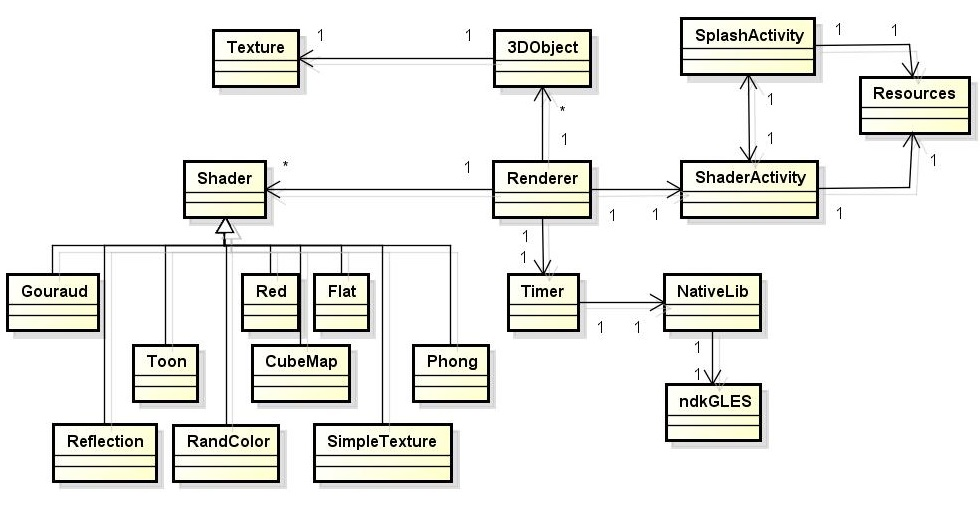
\includegraphics[keepaspectratio=true,scale=0.6]{figuras/class_diagram.jpg}
	\caption{Diagrama de Classe da Implementação em \textit{Android}}
	\label{class_diagram}
	\end{figure}

	\subsection{Classes \textit{Shader Activity} e \textit{Splash Activity}}

	\begin{figure}[h]
	\centering
		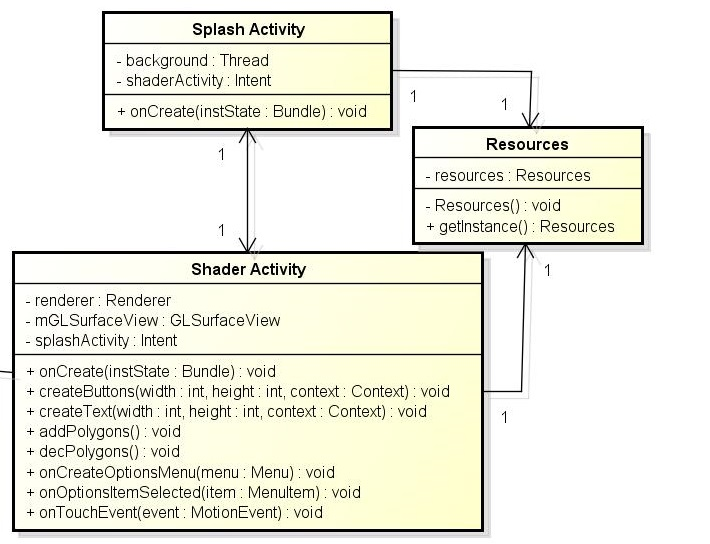
\includegraphics[keepaspectratio=true,scale=0.6]{figuras/shader_splash.jpg}
	\caption{Detalhamento das classes \textit{Shader Activity}, \textit{Splash Activity} e \textit{Resources}}
	\label{shader_splash}
	\end{figure}

	De acordo com \ref{androidsdkmanager}, a plataforma \textit{Android} utiliza o termo \textit{Activity} para descrever a tela de \textit{front-end} da aplicação que interage com o usuário. Ela possui elementos de \textit{design} como texto, botões, gráficos, entre outros. No contexto deste trabalho, há duas classes \textit{Activity}, a \textit{Shader} e a \textit{Splash}. 

	A \textit{Splash Activity} (Figura  \ref{splash_act}) é responsável pela visualização da tela de \textit{loading} enquanto carrega os recursos necessários para o programa (como a leitura dos modelos tridimensionais em formato obj e das imagens usadas para texturização) por meio do uso de \textit{thread}. Estes recursos são setados por meio da classe chamada \textit{Resources}, que utiliza o padrão de projeto chamado \textit{Singleton}, que garante a existencia de apenas uma instância da classe, que será acessada posteriormente.

	\begin{figure}[h]
	\centering
		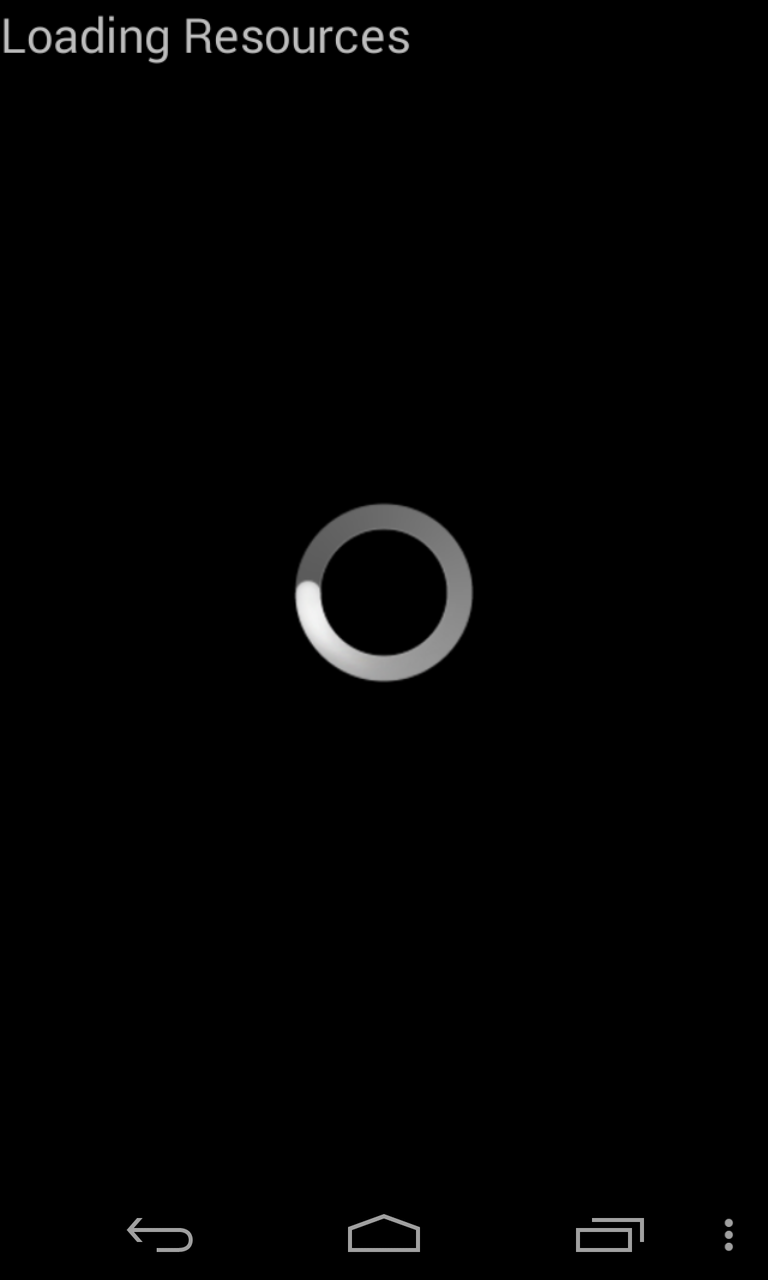
\includegraphics[keepaspectratio=true,scale=0.2]{figuras/splash_act.png}
	\caption{Tela da \textit{Splash Activity}}
	\label{splash_act}
	\end{figure}

	A \textit{Shader Activity} (Figura  \ref{shader_act}) é responsável pela  instanciação da classe \textit{Renderer}, que renderiza os gráficos tridimensionais utilizando a biblioteca \textit{OpenGL ES}. Além disso, ela controla os eventos de \textit{touch}, que permitem escalar e mover o objeto, além de disponibilizar os menus que trocam de \textit{shaders}, os botões que aumentam, diminuem o número de polígonos, a informação do tempo de renderização e a de quantidade de polígonos. Aumenta-se o número de polígonos por meio da troca de objetos que possuem arquivos obj diferentes, que já foram carregados pela \textit{Splash Activity}. 

	\begin{figure}[h]
	\centering
		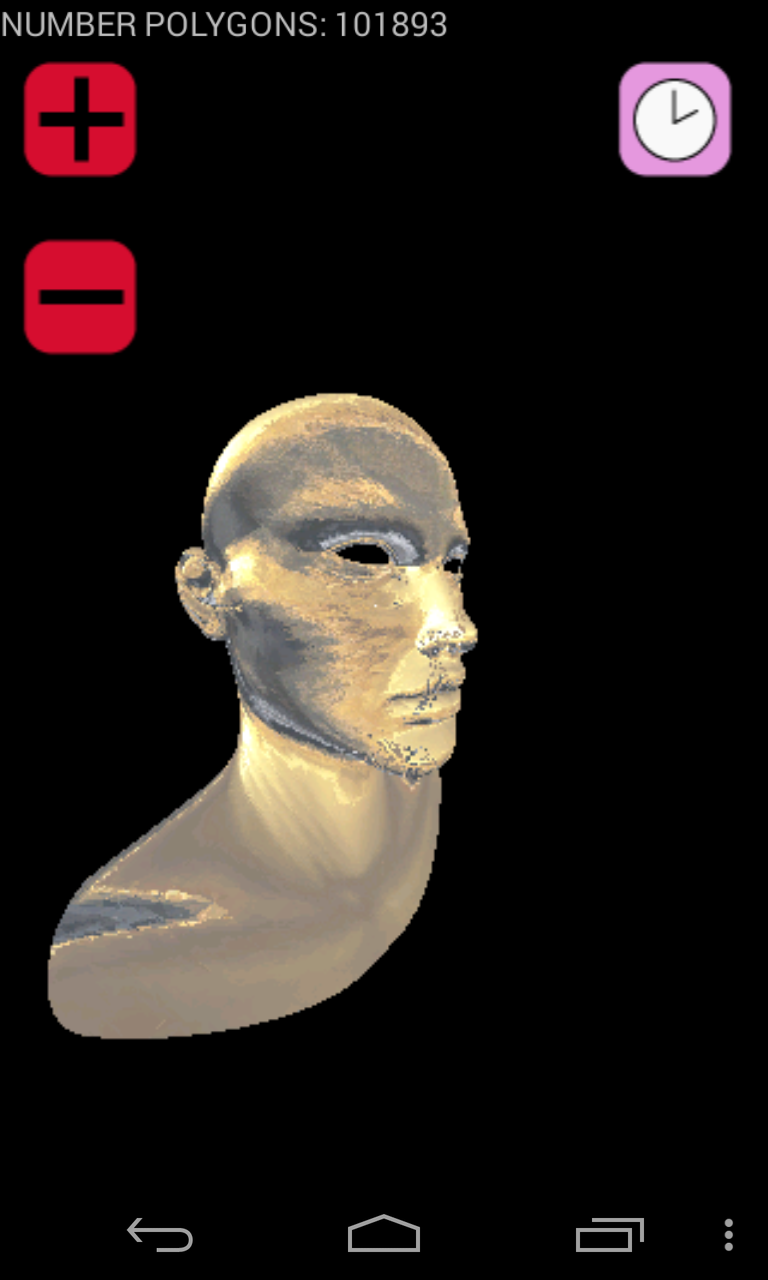
\includegraphics[keepaspectratio=true,scale=0.2]{figuras/shader_act.png}
	\caption{Tela da \textit{Shader Activity}}
	\label{shader_act}
	\end{figure}

	Devido à limitação de memória do dispositivo móvel e os vários objetos com diferentes números de polígonos, não é possível carregar todos de uma só vez. Assim, foi necessário dividir esta quantidade objetos por vez, em que quando chega-se ao último objeto (tanto adicionando, quanto decrementando), volta-se novamente para a \textit{Splash Activity}, a fim de carregar os novos objetos e ir novamente para a \textit{Shader Activity}, a fim de renderizá-los.

	\subsection{ Classes \textit{3DObject} e \textit{Texture}}   

	\begin{figure}[h]
	\centering
		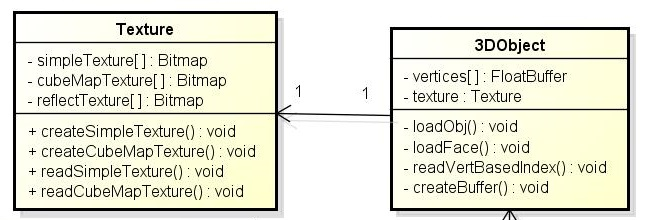
\includegraphics[keepaspectratio=true,scale=0.6]{figuras/object_texture.jpg}
	\caption{Detalhamento das classes \textit{3DObject} e \textit{Texture}}
	\label{object_texture}
	\end{figure}

	A classe \textit{3DObject}, mostrada na Figura \ref{object_texture}, é responsável por ler o arquivo obj e armazenar, em um \textit{buffer}, os vértices de posição, normal e textura na ordem em que será renderizado. No \textit{buffer} cada coordenada relacionada a um vértice (posição, normal e textura) é armazenada alternadamente, como mostra a Figura \ref{buffer}.

	A classe \textit{Texture} cria as texturas utilizadas pelos \textit{shaders} \textit{SimpleTexture}, \textit{CubeMap} e \textit{Reflection}. Para gerar uma textura simples, primeiramente gera-se um objeto de textura \texttt{glGenTextures}, depois vincula-se a a textura a este objeto utilizando a função \texttt{glBindTexture} e carrega-se a imagem por meio da função \texttt{texImage2D}.  Para as texturas do \textit{CubeMap} e \textit{Reflection}, faz-se a mesma coisa, exceto que a função \textit{texImage2D} é feita seis vezes, em que cada textura representa uma face de um cubo. 

	\begin{figure}[h]
	\centering
		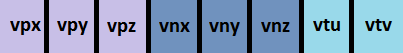
\includegraphics[keepaspectratio=true,scale=1.0]{figuras/buffer.png}
	\caption{Ordem das coordenadas de posição, normal e textura para um vértice}
	\label{buffer}
	\end{figure}

	\subsection{Classes \textit{Timer} e \textit{NativeLib}}      

	\begin{figure}[h]
	\centering
		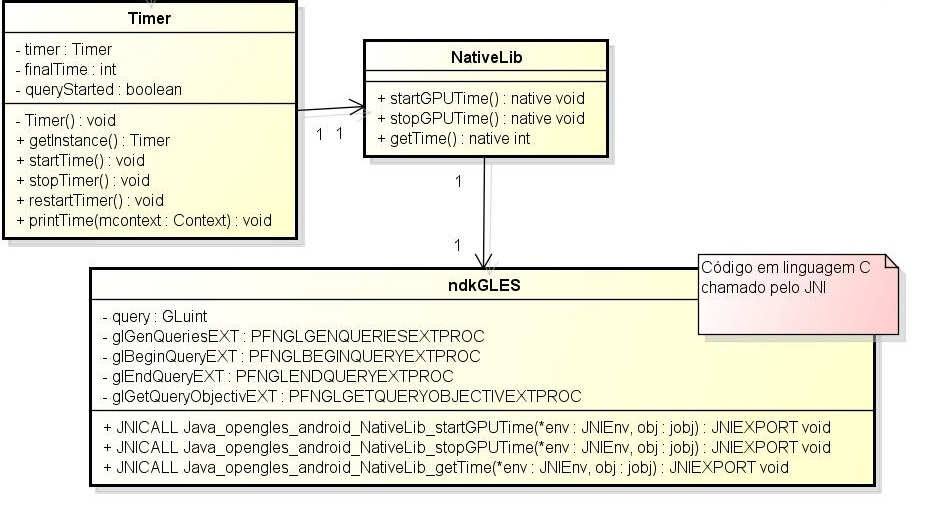
\includegraphics[keepaspectratio=true,scale=0.6]{figuras/timer_nativelib.jpg}
	\caption{Detalhamento das classes \textit{Timer} e \textit{NativeLib}}
	\label{timer_nativelib}
	\end{figure}

	A Figura \ref{timer_nativelib} detalha a classe \textit{Timer}, que realiza a média de dez medições do tempo (em nanosegundos) para cada objeto tridimensional, utilizando um \textit{shader} específico. Cada medição é feita utilizando a linguagem C e a extensão de \textit{OpenGL ES} chamada GL\_EXT\_disjoint\_timer\_query citada na Seção \ref{gpu}.  A integração entre o codigo em linguagem C e o código em Java é feita por meio da classe \textit{NativeLib}.

	\subsection{Classe \textit{Renderer}}    

	\begin{figure}[h]
	\centering
		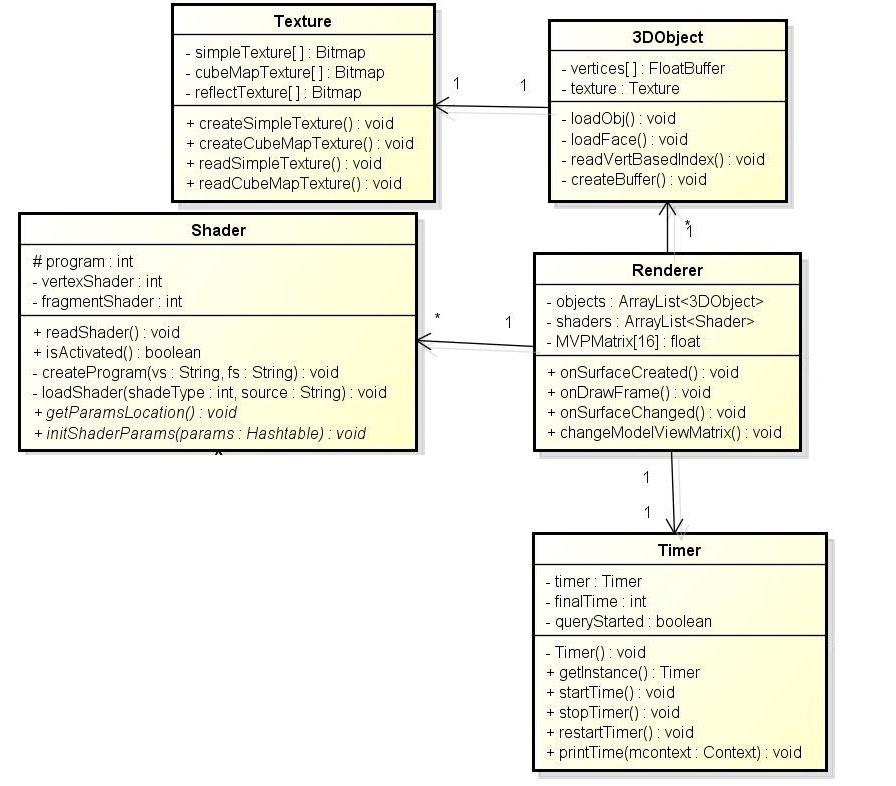
\includegraphics[keepaspectratio=true,scale=0.6]{figuras/renderer.jpg}
	\caption{Detalhamento da classe \textit{Renderer}}
	\label{renderer}
	\end{figure}

	A classe \textit{Renderer} (Figura \ref{renderer}) funciona como uma controladora, sendo o ponto principal  das chamadas provenientes da \textit{view} (\textit{ShaderActivity}) para a camada mais abaixo (\textit{3DObject}, \textit{Shader} e \textit{Timer}). Ela que implementa as funções da biblioteca \textit{OpenGL ES} \texttt{onSurfaceCreated},  \texttt{onDrawFrame} e \texttt{onSurfaceChanged}. A primeira função é chamada apenas uma vez quando a \textit{view} da \textit{OpenGL ES} é instanciada, em que faz-se todas as configurações nesta função, como por exemplo, criação de texturas. A segunda função é chamada em \textit{loop}, em que faz-se a renderização por meio da função \texttt{glDrawArrays}. 

	\subsection{Classe \textit{Shader}}      

	\begin{figure}[h]
	\centering
		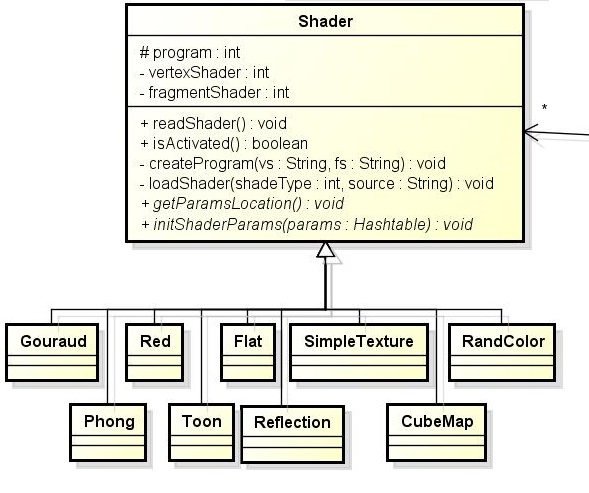
\includegraphics[keepaspectratio=true,scale=0.6]{figuras/shaders_diag.jpg}
	\caption{Detalhamento da classe \textit{Shader}}
	\label{shaders_diag}
	\end{figure}

	A classe \textit{Shader} (Figura \ref{shaders_diag}) é responsável por ler, fazer o \textit{attach} e o \textit{link} do \textit{ vertex} e do \textit{fragment shaders}. Além disso, ela possui os métodos abstratos \texttt{getParamsLocation} e \texttt{initShaderParams(Hastable params)}. Assim, todos os \textit{shaders} que herdam desta classe, são obrigados a implementar estes métodos. O primeiro método faz o armazenamento da localização de cada variável especificada dentro do \textit{shader}, já o segundo método inicializa estas variáveis por meio de um \textit{hash} que é passado como um parâmetro pela classe \textit{Renderer}.     

	\subsection{ \textit{Shaders} Implementados}    

	A fim de de poder fazer a análise da complexidade algorítmica, alguns \textit{shaders} foram implementados, em que cada um deles herdam da classe \textit{Shader} e implementam seus métodos abstratos. Estes \textit{shaders} podem ser vistos na Figura \ref{shaders_impl}.  

	\begin{figure}[h]
	\centering
		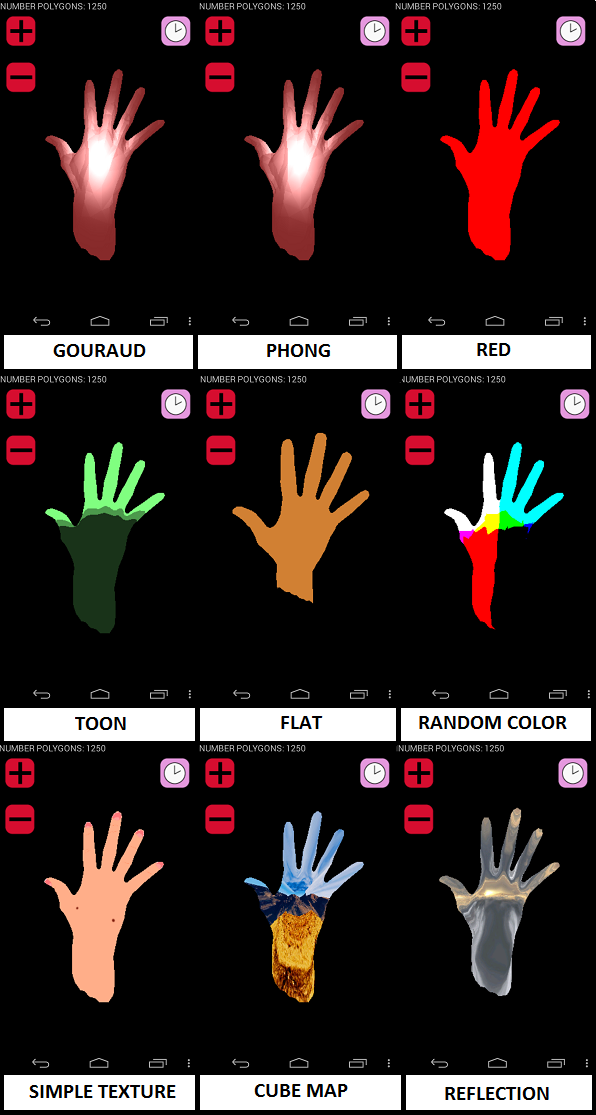
\includegraphics[keepaspectratio=true,scale=0.7]{figuras/shaders_impl.png}
	\caption{\textit{Shaders} Implementados}
	\label{shaders_impl}
	\end{figure}


\section{Plotagem e Aplicação do Método dos Mínimos Quadrados}

	Para a plotagem e aplicação do método dos mínimos quadrados, foi feito um programa em linguagem \textit{Python}, a fim de automatizar este processo. O programa encontra-se estruturado de acordo com a Figura \ref{minquad_diag}, em que a classe \textit{ReadCSV} é responsável por ler os arquivos CSV e fazer a média das métricas tanto para o \textit{vertex shader} como para o \textit{fragment shader}. Já a classe \textit{PlotChart}, faz a plotagem do gráfico do número de instruções por segundo por vértice \textit{versus} o número de polígonos e do gráfico do número de instruções por segundo por fragmento \textit{versus} o número de polígonos. Além disso, ele também plota o gráfico original juntamente com o gráfico após a aplicação do método dos mínimos quadrados. Por fim, o módulo \textit{LeastSquares} realiza o ajuste dos mínimos quadrados para uma reta e para polinômios de segundo e terceiro graus como explicado na Seção \ref{metminqua}. Ele também calcula os erros associados a cada ajuste e indica qual o menor. 

	\begin{figure}[h]
	\centering
		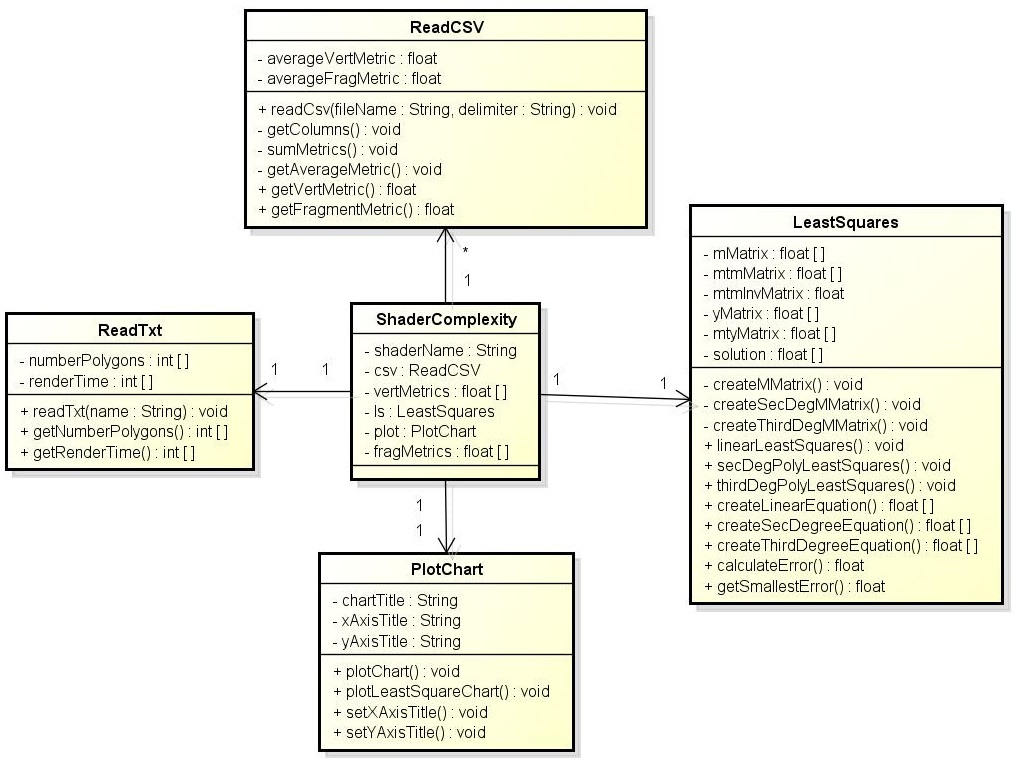
\includegraphics[keepaspectratio=true,scale=0.6]{figuras/minquad_diag.jpg}
	\caption{Diagrama de Classes do código de automatização}
	\label{minquad_diag}
	\end{figure}


\section{Análise Numérica}


